%
%%\part{高级系统管理}
%
%
%\section{系统安装}
%
%
%\subsection{分区的考虑}
%
%
%\subsection{安装过程的监控}
%
%
%\subsection{非标准安装方法}
%
%
%\begin{frame}{Kickstart:自动化安装}
%\begin{itemize}
%\item 脚本化安装方法
%\item 支持所有的Anaconda 特性
%\item /root/ananconda-ks.cfg 是安装过程中自动创建的配置文件
%\item 配置工具:system-config-kickstart
%\item 语法检查: ksvalidator
%\end{itemize}
%
%\end{frame} 
%
%\begin{frame}{开始Kickstart安装}
%\begin{itemize}
%\item 启动时,输入ks参数告诉Anaconda进入Kickstart模式
%\item ks 查询DHCP来获得Kickstart的位置
%\item ks=url 通过http,ftp 或NFS获得配置文件
%\item 从本地介质获得:
%
%\begin{itemize}
%\item ks=floppy
%\item ks=cdrom
%\item ks=hd:\emph{device:/path/to/file}
%\end{itemize}
%\end{itemize}
%
%\end{frame} 
%\begin{frame}{Kickstart文件剖析}
%\begin{itemize}
%\item Command Section
%
%\begin{itemize}
%\item 配置系统
%\item 传递提示给用户的指令
%\end{itemize}
%\item \%packages section
%
%\begin{itemize}
%\item 选择安装的包和组
%\item 依赖性通常已经解决了
%\end{itemize}
%\item Scripts section(s)
%
%\begin{itemize}
%\item 可选的部分,用来定制系统
%\item \%pre 脚本是在安装前运行
%\item \%post 脚本是安装后运行
%\end{itemize}
%\end{itemize}
%
%\end{frame} 
%\begin{frame}{Kickstart:Commands Section}
%\begin{itemize}
%\item 安装模式
%
%\begin{description}
%\item [{install}] 全新安装
%\item [{upgrade}] 升级现有安装
%\end{description}
%\item 安装方法
%
%\begin{itemize}
%\item cdrom
%\item url --url \emph{url}
%\item nfs --server \emph{host }--path \emph{directory}
%\item harddrive --partition=\emph{device} --dir=\emph{/path/to/install\_tree}
%\end{itemize}
%\end{itemize}
%
%\end{frame} 
%\begin{frame}{Kickstart: Commands section 重要指令}
%\begin{itemize}
%\item 必须的指令
%
%\begin{itemize}
%\item 这些指令是必须的,否则安装程序会要求用户干预配置
%\item 本地化选项:keyboard,lang,timezone
%\item 认证: rootpw,authconfig
%\item 引导:bootloader
%\end{itemize}
%\item 可选指令
%
%\begin{itemize}
%\item 网络: network {[} options {]}
%\item 安全:firewall,selinux,services
%\item 安装程序行为:firstboot,poweroff | reboot,interactive,text
%\end{itemize}
%\end{itemize}
%
%\end{frame} 
%\begin{frame}{Kickstart:Packages Section}
%\begin{itemize}
%\item 用 package\_name 增加单个包,不需要任何版本参数,只要包的名称
%\item @package\_group 增加一组包
%\item -package\_name 从列表中删除包
%\item 可以用通配符指定多个包
%\item 通常已经解决依赖关系
%\item @lang-support 为额外的语言增加支持
%\item key 指令指定的话,分层产品的包将会安装
%\end{itemize}
%
%\end{frame} 
%\begin{frame}{Kickstart:\%pre, \%post}
%\begin{itemize}
%\item \%pre 安装要做的事情
%
%\begin{itemize}
%\item 作为bash脚本执行
%\item Kickstart文件分析后执行
%\end{itemize}
%\item \%post 安装要做的事情
%
%\begin{itemize}
%\item 可以指定解释器(缺省是bash)
%\item 缺省是chroot环境,不过可以不在chroot下执行
%\end{itemize}
%\end{itemize}
%\end{frame} 
%



\section{高级文件系统管理}

\begin{frame}{高级文件系统管理}
	\tableofcontents[currentsection]
\end{frame}

%\subsection{使用配额}
%
%
%\begin{frame}{配置文件系统配额}
%\begin{itemize}
%\item 概述
%
%\begin{itemize}
%\item 由内核实现
%\item 做为每一个文件系统的基本功能而内置
%\item 针对每一个用户或者组设定独立的策略
%
%\begin{itemize}
%\item 限定块或者inode的数量
%\item 实现soft和hard两个类型限制
%\end{itemize}
%\end{itemize}
%\item 初始化
%
%\begin{itemize}
%\item 挂载文件系统增加usrquota,grpquota选项
%\item 初始化配额数据库: quotacheck
%\end{itemize}
%\end{itemize}
%
%\end{frame} 
%\begin{frame}{为用户设置配额}
%
%实现
%\begin{itemize}
%\item 启动或停止配额:quotaon,quotaoff
%\item 直接编辑配额:edquota \emph{username}
%\item 命令直接设置:\\
%setquota \emph{username} 4096 5120 40 50 /foo
%\item 定义配额模板\\
%edquota -p \emph{user1 user2}
%\end{itemize}
%
%\end{frame} 
%\begin{frame}{配额状态报告}
%\begin{itemize}
%\item 用户检查:quota
%\item 配额概览:repquota
%\item 其他工具:warnquota
%\end{itemize}
%\end{frame} 

\subsection{RAID概述}
\begin{frame}{RAID概述}

独立磁盘冗余阵列(RAID, Redundant Array of Independent Disks)简称磁盘阵列,其基本思想就是把多个相对便宜的硬盘组合起来,成为一个磁盘阵列组,使性能达到甚至超过一个价格昂贵、容量巨大的硬盘\footnote{http://zh.wikipedia.org/wiki/RAID}

优点:
\begin{itemize}
\item 增强资料整合度
\item 增强容错功能
\item 增加处理量或容量
\end{itemize}
\end{frame}

\begin{frame}{RAID0}
\begin{columns}
\column{2cm}

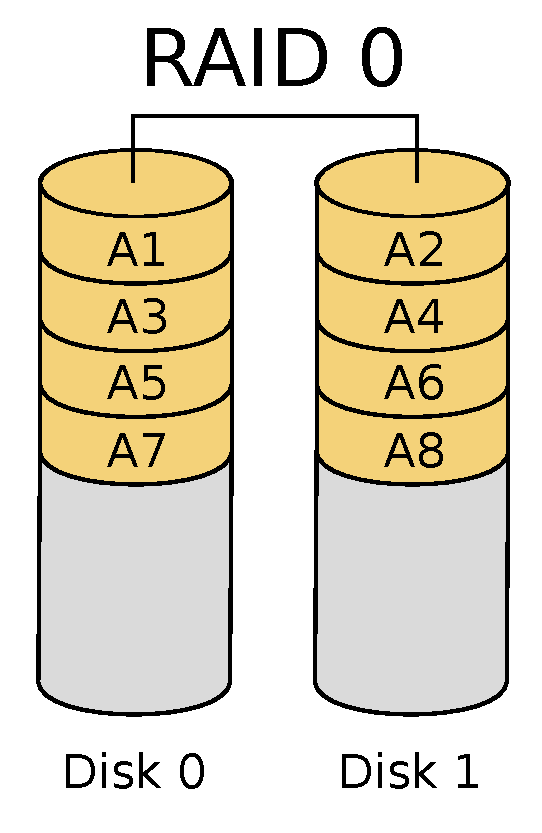
\includegraphics[scale=.4]{RAID_0}

\column{5cm}
将多个磁盘合并成一个大的磁盘,不具有冗余,并行I/O,速度最快。RAID 0亦称为带区集。

%$size = 2 x min(S_1,S_2)$
\end{columns}
\end{frame}

\begin{frame}{RAID1}
\begin{columns}
\column{2cm}
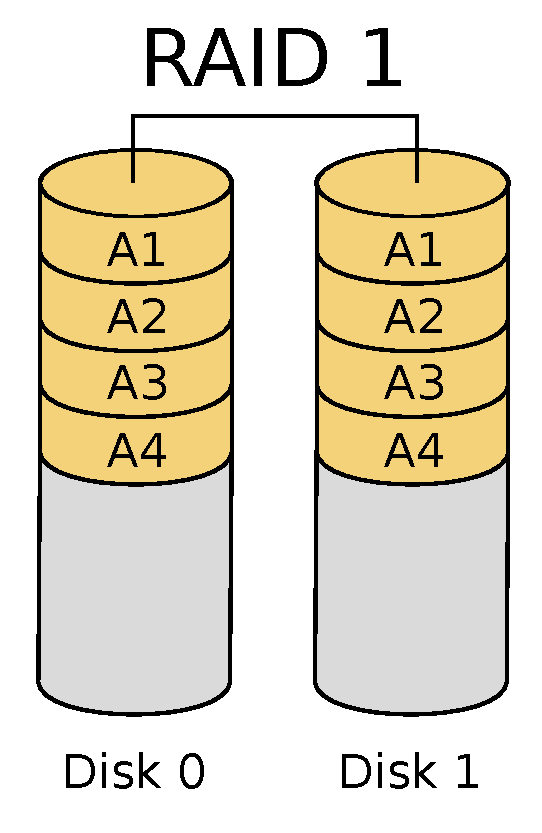
\includegraphics[scale=.4]{RAID_1}

\column{5cm}

两组以上的N个磁盘相互作镜像,在一些多线程操作系统中能有很好的读取速度,另外写入速度有微小的降低。除非拥有相同资料的主磁盘与镜像同时损坏,否则只要一个磁盘正常即可维持运作,可靠性最高。

%$size= min(S_1,S_2)$
\end{columns}
\end{frame}

%\begin{frame}{RAID2}
%\includegraphics{RAID_2}
%
%这是RAID 0的改良版,以汉明码(Hamming Code)的方式将数据进行编码后分割为独立的位元,并将数据分别写入硬盘中。因为在数据中加入了错误修正码(ECC,Error Correction Code),所以数据整体的容量会比原始数据大一些,RAID2最少要三块磁盘方能运作。
%\end{frame}

\begin{frame}{RAID3}

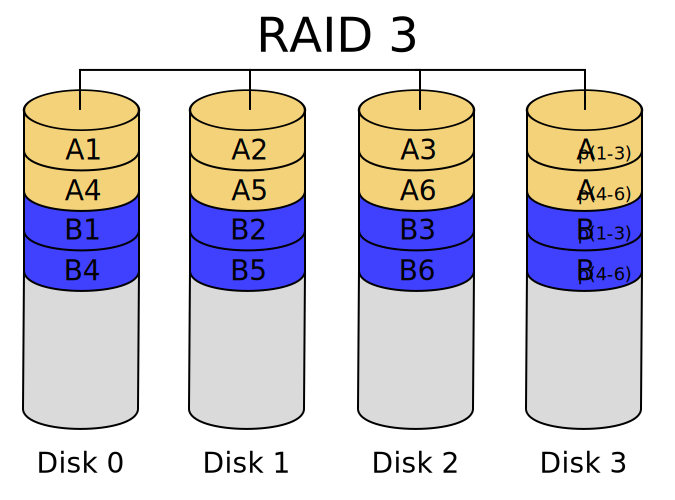
\includegraphics[scale=.4]{RAID_3}

采用Bit-interleaving(数据交错储存)技术,它需要通过编码再将数据位元分割后分别存在硬盘中,而将同位元检查后单独存在一个硬盘中,这种规格比较适于读取大量数据时使用。

\end{frame}

%\begin{frame}{RAID4}
%
%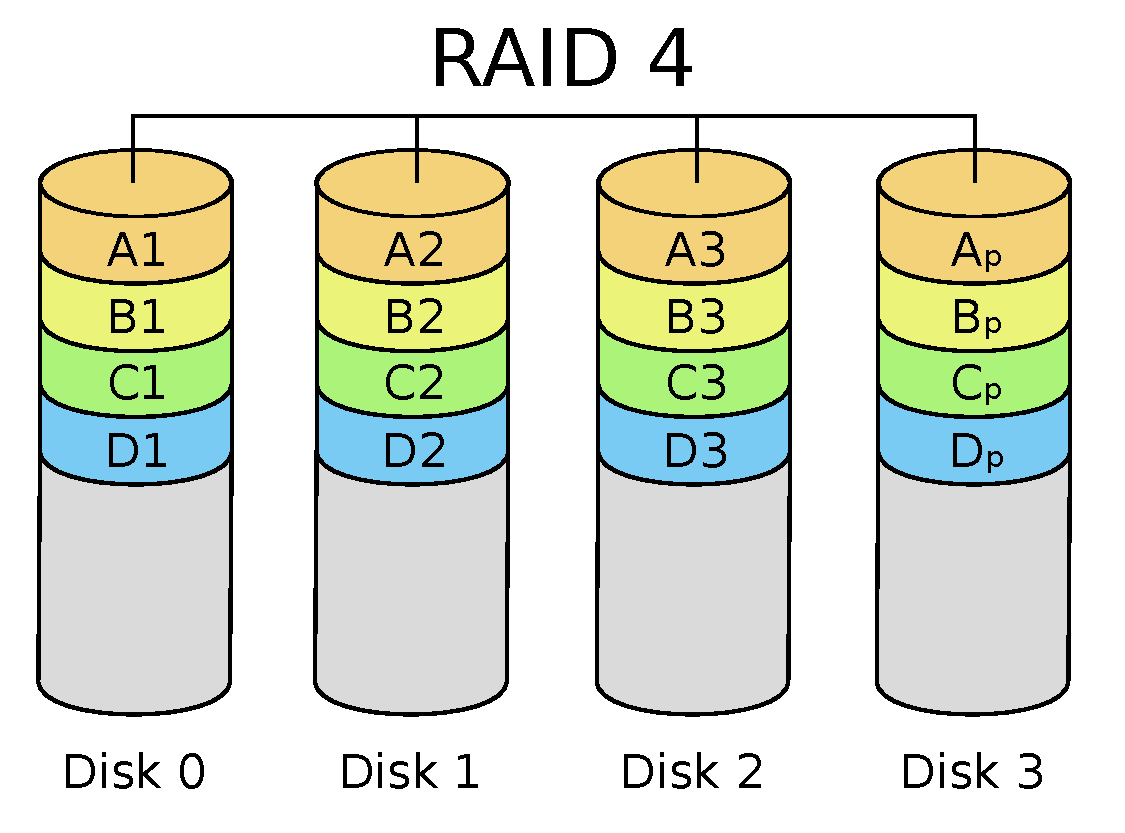
\includegraphics[scale=.4]{RAID_4}
%
%它与RAID 3不同的是它在分割时是以区块为单位分别存在硬盘中,但每次的数据存取都必须从同位元检查的那个硬盘中取出对应的同位元数据进行核对,由于过于频繁的使用,所以对硬盘的损耗可能会提高
%
%
%\end{frame}


\begin{frame}{RAID5}

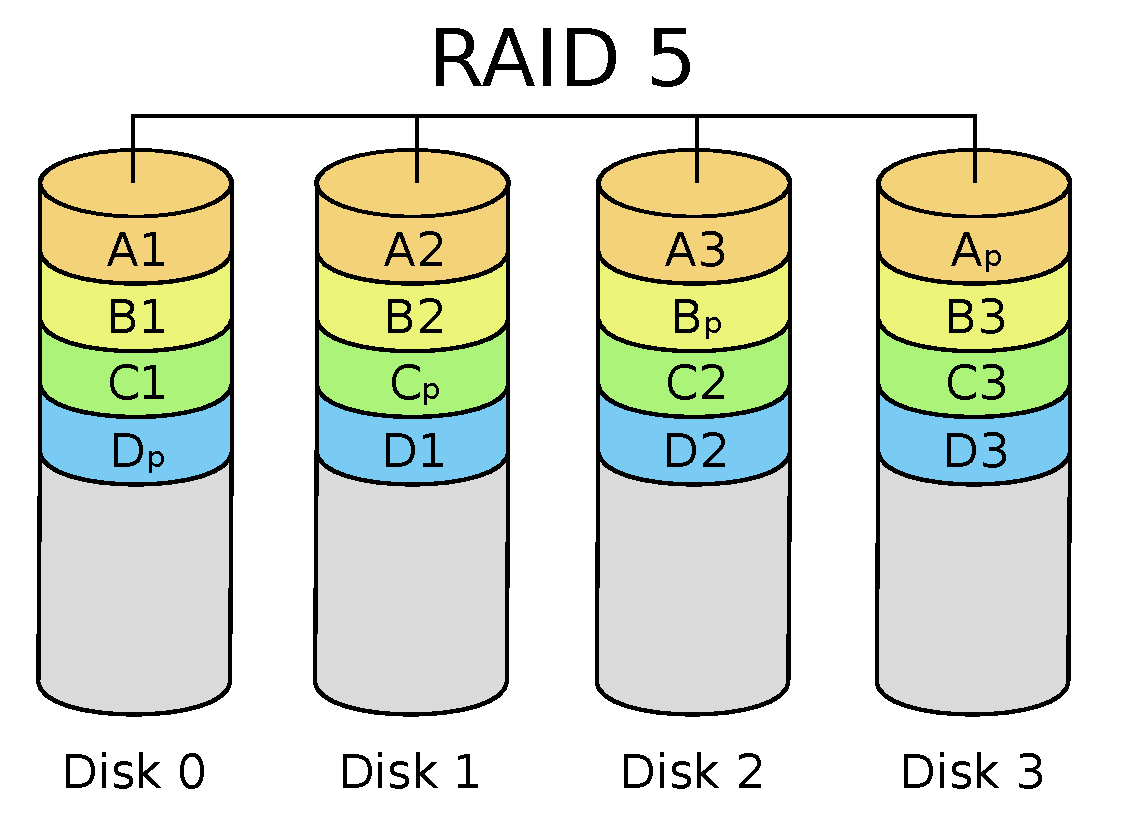
\includegraphics[scale=.4]{RAID_5}


RAID 5 是一种存储性能、数据安全和存储成本兼顾的存储解决方案。它使用的是Disk Striping(硬盘分割)技术。 把数据和相对应的奇偶校验信息存储到组成RAID5的各个磁盘上.并且奇偶校验信息和相对应的数据分别存储于不同的磁盘上。

%$Size = (N -1 ) * min(S_1,S2,\ldots,S_N)$

\end{frame}

\begin{frame}{RAID6}

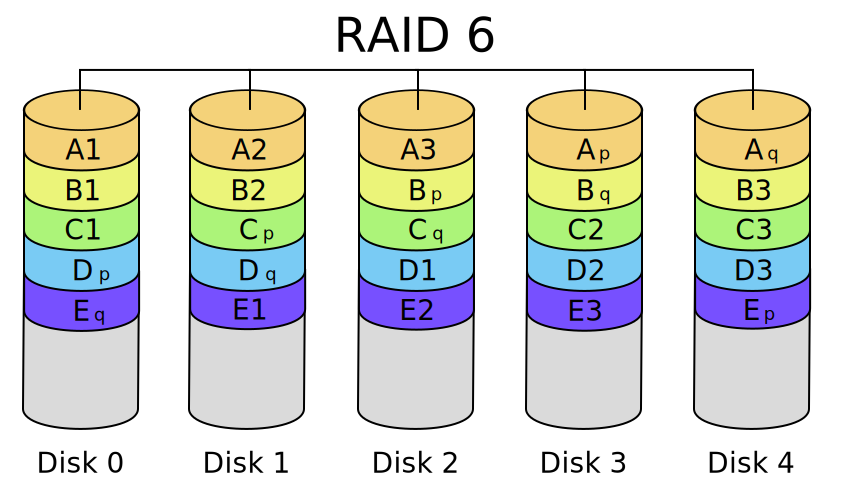
\includegraphics[scale=.4]{RAID_6}


RAID 6相比RAID 5增加了第二个独立的奇偶校验信息块。两个独立的奇偶系统使用不同的算法,数据的可靠性非常高,但相对于RAID 5有更大的“写损失”,因此“写性能”非常差。较差的性能和复杂的实作方式使得RAID 6很少得到实际应用。


\end{frame}

\begin{frame}{RAID10/01}
RAID 1+0是先镜射再分割资料。是将所有硬盘分为两组,视为是RAID 0的最低组合,然后将这两组各自视为RAID 1运作。RAID 1+0有着不错的读取速度,而且拥有比RAID 0更高的资料保护性。 \\
RAID 0+1则是跟RAID 1+0的程序相反,是先分割再将资料镜射到两组硬盘。它将所有的硬盘分为两组,变成RAID 1的最低组合,而将两组硬盘各自视为RAID 0运作。RAID 0+1比起RAID 1+0有着更快的读写速度,不过也多了一些会让整个硬盘组停止运转的机率;因为只要同一组的硬盘全部损毁,RAID 0+1就会停止运作,而RAID 1+0则可以在牺牲RAID 0的优势下正常运作。 \\
至少必须拥有四个以上的偶数硬盘才能使用。
\end{frame}
\subsection{使用软RAID}

\begin{frame}{什么是软RAID}
\begin{itemize}
\item 相比硬件RAID而言,RAID实现由系统完成,而不是RAID卡的固件
\item mdadm 提供了软RAID的管理接口
\item 支持多种RAID级别,包括RAID 0,1,5
\item 支持备用磁盘来增加额外的冗余度
\item RAID设备命名为/dev/md0,/dev/md1,以此类推
\end{itemize}

\end{frame} 

\begin{frame}{软RAID配置}
\begin{itemize}
\item 使用mdadm创建和定义RAID\\
mdadm -C /dev/md0 -a yes -l 1 -n 2 -x 1 /dev/sda1 /dev/sdb1 /dev/sdc1
\item 格式化每一个RAID设备\\
mkfs.ext3 /dev/md0
\item 测试RAID设备
\item mdadm还可以检查RAID设备的状态\\
mdadm --detail /dev/md0
\end{itemize}

\end{frame} 

\begin{frame}{软RAID测试及恢复}
\begin{itemize}
\item 模拟磁盘故障\\
mdadm /dev/md0 -f /dev/sda1
\item 从软RAID磁盘故障中恢复

\begin{itemize}
\item 替换有故障的磁盘
\item 对硬盘进程分区等操作,获得和故障硬盘一样的分区结构
\item mdadm /dev/md0 -a /dev/sda1
\end{itemize}
\item mdadm,/proc/mdstat,/var/log/\{dmesg,messages\}
\item 软RAID遵循RAID规范和限定
\end{itemize}
\end{frame} 
\subsection{使用逻辑卷管理(LVM)}

\begin{frame}{什么是LVM}
\begin{itemize}
\item LVM=Logical Volume Manager
\item 方便处理卷的一个抽象层,包括文件系统的大小更改
\item 允许跨物理设备来组织文件系统

\begin{itemize}
\item 物理设备被当作物理卷 (Physical Volumes, PV)
\item 一个或者多个物理卷组成卷组( Volume Group,VG)
\item 物理卷由固定大小的物理段(Physical Extents,PE)
\item 逻辑卷(Logical Volume,LV)在物理卷上创建,由物理段组成
\item 在逻辑卷上创建文件系统
\end{itemize}
\end{itemize}
\end{frame}

\begin{frame}[plain]{LVM逻辑结构}

\includegraphics[scale=0.5]{lvm.pdf}
\end{frame} 

\begin{frame}{创建逻辑卷(LV)}

\begin{itemize}
\item 创建物理卷\\
pvcreate /dev/hda3
\item 将物理卷分配到卷组\\
vgcreate vg0 /dev/hda3
\item 从特定卷组里创建逻辑卷\\
lvcreate -L 256M -n data vg0\\
mkfs.ext3 /dev/vg0/data 
\item rflvm/system-config-lvm 图形化的配置工具
\end{itemize}

\end{frame} 
\begin{frame}{更改逻辑卷大小}
\begin{itemize}
\item 增大卷

\begin{itemize}
\item lvextend可以增大逻辑卷
\item resize2fs可以在线加大EXT3文件系统
\item vgextend增加新的物理卷到某一个卷组里
\end{itemize}
\item 缩小卷

\begin{itemize}
\item 首先文件系统必须减小
\item 必须\alert{离线}做文件系统检查
\item lvreduce可以减小逻辑卷
\item 卷组可以通过下面的方法减小

\begin{itemize}
\item pvmove /dev/hda3
\item vgreduce vg0 /dev/hda3
\end{itemize}
\end{itemize}
\end{itemize}

\end{frame} 

\begin{frame}{逻辑卷快照}
\begin{itemize}
\item 快照(Snapshot)是一个特殊的逻辑卷,它是在快照生成的时间点对某一个逻辑卷的精确拷贝
\item 采取写时复制技术(Copy on Write, CoW)
\item 快照一般用来执行备份和对某一个数据集的临时拷贝
\item 快照仅仅消耗从快照创建开始,原始卷发生改变需要存储的空间

\begin{itemize}
\item 快照在创建是分配空间,但是并不使用,直到原始卷有改变
\item 当发生改变时,原始卷上老的数据被拷贝到快照上
\end{itemize}
\item \href{http://blog.wgzhao.com/2008/06/20/LVM-snapshot-on.html}{http://blog.wgzhao.com/2008/06/20/LVM-snapshot-on.html}
\end{itemize}
\end{frame}

\begin{frame}[plain]{逻辑卷快照原理图}
\includegraphics[scale=0.6]{lvm-snapshot.pdf}
\end{frame} 

\begin{frame}{使用快照}
\begin{itemize}
\item 对某一个逻辑卷做快照\\
lvcreate -l 30 -s -n backup /dev/vg0/data
\item 挂载快照\\
mkdir -p /mnt/backup\\
mount -o ro /dev/vg0/backup /mnt/backup
\item 删除快照\\
umount /mnt/backup \\
lvremove /dev/vg0/backup
\end{itemize}
\end{frame} 

\subsection{/proc 文件系统}

\begin{frame}{什么是proc文件系统}
在许多类 Unix 计算机系统中, procfs 是 进程 文件系统 (file system) 的缩写,包含一个伪文件系统(启动时动态生成的文件系统),用于通过内核访问进程信息。这个文件系统通常被挂载到 /proc 目录。由于 /proc 不是一个真正的文件系统,它也就不占用存储空间,只是占用有限的内存。
除Linux外,Solaris,BSD,IBM AIX,QNX等均支持proc文件系。
\end{frame}

\begin{frame}{/proc/scsi}
作为系统管理员,需要了解的最有用内容是,在有热插拔硬盘情况下,如何不重启系统就可以添加更多磁盘空间。这里,可以用以下命令来使系统识别新的磁盘:

echo “scsi add-single-device w x y z” > /proc/scsi/scsi

为使该命令正常运行,必须指定正确的参数值 w、x、y 和 z,如下所示:\\
w 是主机适配器(HBA)标识,第一个适配器为零(0) \\
x 是主机适配器上的 SCSI 通道,第一个通道为零(0) \\
y 是设备的 SCSI 标识 \\ 
z 是 LUN 号,第一个 LUN 为零(0) \\


相反的,在不重新引导系统的情况下将设备从系统中除去的命令是:

echo “scsi remove-single-device w x y z” > /proc/scsi/scsi

\end{frame}

\begin{frame}{/proc/sys/fs/}
\begin{exampleblock}{file-max}
该文件指定了可以分配的文件句柄的最大数目。如果用户得到的错误消息声明由于打开文件数已经达到了最大值,从而他们不能打开更多文件,则可能需要增加该值。可将这个值设置成有任意多个文件,并且能通过将一个新数字值写入该文件来更改该值。
\end{exampleblock}

\begin{exampleblock}{file-nr}
该文件与 file-max 相关,它有三个值:
已分配文件句柄的数目
已使用文件句柄的数目
文件句柄的最大数目
该文件是只读的,仅用于显示信息.
\end{exampleblock}

\end{frame}



\begin{frame}{/proc/sys/kernel/}
\begin{description}
\item[hostname] 允许您配置网络主机名。它没有缺省值,也许已经设置了主机名,也许没有设置。
\item[msgmax] 指定了从一个进程发送到另一个进程的消息的最大长度。进程间的消息传递是在内核的内存中进行,不会交换到磁盘上,所以如果增加该值,则将增加操作系统所使用的内存数量。
\item[msgmnb] 指定在一个消息队列中最大的字节数。
\item[msgmni] 指定消息队列标识的最大数目。
\item[panic] 表示如果发生kernel panic 则内核在重新引导之前等待的秒数。0 将禁止重新引导。
\item[shmall] 该文件是在任何给定时刻系统上可以使用的共享内存的总量(以字节为单位)。
\item[shamax] 该文件指定内核所允许的最大共享内存段的大小(以字节为单位)。
\item[shmmni] 该文件表示用于整个系统共享内存段的最大数目
\item[sysrq] 如果该文件指定的值为非零,则激活 System Request Key。
\item[threads-max]  该文件指定内核所能使用的线程的最大数目。
\end{description}
\end{frame}


\begin{frame}{/proc/sys/net/core}
\begin{description}
%\item[message\_burst] 写新的警告消息所需的时间(以 1/10 秒为单位);在这个时间内所接收到的其它警告消息会被丢弃。这用于防止某些企图用消息“淹没”您系统的人所使用的拒绝服务(Denial of Service)攻击。
%\item[message\_cost] 该文件存有与每个警告消息相关的成本值。该值越大,越有可能忽略警告消息。
%\item[netdev\_max\_backlog] 该文件指定了,在接口接收数据包的速率比内核处理这些包的速率快时,允许送到队列的数据包的最大数目。
\item[optmem\_max] 该文件指定了每个套接字所允许的最大缓冲区的大小。

\item[rmem\_default] 该文件指定了接收套接字缓冲区大小的缺省值(以字节为单位)。

\item[rmem\_max] 该文件指定了接收套接字缓冲区大小的最大值(以字节为单位)。

\item[wmem\_default] 该文件指定了发送套接字缓冲区大小的缺省值(以字节为单位)。

\item[wmem\_max] 该文件指定了发送套接字缓冲区大小的最大值(以字节为单位)。
\end{description}
\end{frame}

\begin{frame}{/proc/sys/net/ipv4}
所有 IPv4 和 IPv6 的参数都被记录在内核源代码文档中。请参阅文件 \\ /usr/src/linux/Documentation/networking/ip-sysctl.txt。 \\
或者 \\
/usr/share/doc/kernel-doc-<version>/Documentation/networking/ip-sysctl.txt
\end{frame}

\begin{frame}[allowframebreaks]{/proc/sys/vm}

\begin{exampleblock}{buffermem}
用来控制用于缓存区的内存的大小,它有三个值, \\
第一个用于缓冲区的内存的最低百分比 \\
第二个表示如果发生所剩系统内存不多,而且系统内存正在减少这种情况,系统将试图维护缓冲区内存的数量。 \\
第三个用于缓冲区的内存的最高百分比
\end{exampleblock}


\begin{exampleblock}{freepages}
 该文件控制系统如何应对各种级别的可用内存。它有三个值 \\
第一个表示如果系统中可用页面的数目达到了最低限制,则只允许内核分配一些内存。 \\
第二个表示如果系统中可用页面的数目低于这一限制,则内核将以较积极的方式启动交换,以释放内存,从而维持系统性能。 \\
第三个表示内核将试图保持这个数量的系统内存可用。低于这个值将启动内核交换。
\end{exampleblock}


\begin{exampleblock}{kswapd}
该文件控制允许内核如何交换内存。它有三个值\\
第一个表示内核试图一次释放的最大页面数目。如果想增加内存交换过程中的带宽,则需要增加该值。\\
第二个表示内核在每次交换中试图释放页面的最少次数。\\
第三个内核在一次交换中所写页面的数目。这对系统性能影响最大。这个值越大,交换的数据越多,花在磁盘寻道上的时间越少。然而,这个值太大会因“淹没”请求队列而反过来影响系统性能。
\end{exampleblock}
\end{frame}

\begin{frame}{修改proc值}
\begin{itemize}
\item echo 重定向,即时生效,重启生效  \\
	echo 1 >/proc/sys/net/ipv4/icmp\_echo\_ignore\_all
\item sysctl 修改/proc/sys下的值,即时生效,重启失效   \\
	sysctl -w net.ipv4.icmp\_echo\_ignore\_all
\item 修改/etc/sysctl.conf,重启后依然有效
\end{itemize}
\end{frame}


\subsection{文件归档}

\begin{frame}{归档工具:tar}
\begin{itemize}
\item tar 可以备份到一个文件或者磁带设备上
\item 支持gzip和bzip2压缩
\item 能保留文件许可,拥有关系和时间戳
\item 支持扩展属性
\item 使用 rmt 指令可以写入到远程磁带设备
\end{itemize}

\end{frame} 
\begin{frame}{归档工具:dump/restore}
\begin{itemize}
\item 备份和恢复ext2/ext3文件系统

\begin{itemize}
\item 其他文件系统目前不支持
\item dump应该仅对没有挂载的或者只读的文件系统操作
\end{itemize}
\item 能做完全或者增量备份
\item 例子\\
dump -0u -f /dev/st0 /dev/hda2\\
restore -rf /dev/st0
\end{itemize}

\end{frame} 
\begin{frame}{归档工具:rsync}
\begin{itemize}
\item 高效的文件拷贝,无论是从远程,还是到远程
\item 使用ssh连接来做安全数据传输\\
rysnc {*}.dbf xplore:/data/backup
\item 比scp更快---差异性拷贝
\end{itemize}
\end{frame} 
%\subsection{实验}
%
%\begin{frame}{实验I:配置实现配额}
%
%
%
%要求:用户victor在/home下使用空间不能超过1024K
%
%提示:
%\begin{enumerate}
%\item 创建用户victor
%\item 对/home激活配额
%\item 设置配额值包括soft和hard
%\item 测试
%\end{enumerate}
%
%\end{frame} 
%\begin{frame}{实验II:软RAID实践}
%\begin{description}
%\item [{场景:}] 一个关键应用需要安装在冗余介质上。于是做出了在现有系统上使用软RAID的决定。修改你的系统配置使得支持带热备的镜像阵列
%\item [{要求:}] 带自动失效恢复(auto-fail-over)的RAID 1 系统
%\end{description}
%提示
%\begin{enumerate}
%\item 创建需要的分区或者设备
%\item 使用mdadm
%\item 测试
%\end{enumerate}
%
%\end{frame} 
%\begin{frame}{实验II:逻辑卷操作}
%\begin{description}
%\item [{场景:}]~\end{description}
%\begin{enumerate}
%\item 为了让新创建的RAID能够共享给多个应用,决定在RAID设备上部署LVM。一个逻辑卷需要创建为ext3文件系统。
%\item 需要增加一个卷组来为总是要求额外空间的应用提供服务。创建这个卷组,使其包含两个分区,新的分区能够加入进来,新的文件系统可以扩展
%\item 老的应用程序数据不再增加,通过备份,调整后,需要的空间相比最初少了很多,为了节省空间,需要把空闲的空间分离出来。\end{enumerate}
%\begin{description}
%\item [{要求:}] 创建LVM,并根据需要扩展,缩小逻辑卷大小
%\end{description}
%\end{frame} 
%
%\section{性能调优}
%
%
%\section{虚拟化}
%
%
%\subsection{概述}
%
%
%
%\begin{frame}{虚拟化}
%
%目标
%\begin{itemize}
%\item 什么是虚拟化
%\item 理解Xen技术
%\item 理解KVM技术
%\item 虚拟化工具链
%\item Xen 工具
%\item KVM 工具
%\end{itemize}
%
%\end{frame} 
%\begin{frame}{优势}
%\begin{itemize}
%\item 资源的高效使用
%\item 可管理性
%\item 安全性
%\item 更低的总拥有成本(CTO)
%\end{itemize}
%\end{frame} 
%\subsection{Xen的虚拟化}
%
%
%
%\begin{frame}{Xen的关键概念}
%\begin{itemize}
%\item 超级监控器(Hypervisor)小巧
%\item 第一个域('Domain')管理系统
%\item 支持完全虚拟化和半虚拟化
%\end{itemize}
%
%\end{frame} 
%\begin{frame}{硬件的考虑因素}
%\begin{itemize}
%\item 最低要求
%
%\begin{itemize}
%\item 带PAE支持的CPU
%\item 每一个 Domain 256MB 内存
%\item 每个 Domain 6GB 磁盘空间
%\end{itemize}
%\item 额外的考虑因素
%
%\begin{itemize}
%\item 对于完全虚拟化,需要带VT/SVM功能的CPU支持
%\item 在线迁移的实现有赖于共享存储
%\item 应用程序的不同导致需要的存储空间大小也不同
%\end{itemize}
%\end{itemize}
%
%\end{frame} 
%\begin{frame}{准备Domain-0}
%\begin{itemize}
%\item 安装Domain0(大部分发行版本自带)
%\item 启动Xen Hypervisor
%\item 启动xend 管理守护进程
%\end{itemize}
%
%\end{frame} 
%\begin{frame}{虚拟资源}
%\begin{itemize}
%\item CPU
%
%\begin{itemize}
%\item 使用VCPU (Virtual CPUs)
%\item 不需要直接映射到真实CPU上
%\end{itemize}
%\item 存储
%
%\begin{itemize}
%\item 块设备
%\item 简单文件
%\end{itemize}
%\item 网络设备
%
%\begin{itemize}
%\item 网桥或者到Domain0的路由
%\item 默认是映射到xenbr0设备上
%\end{itemize}
%\end{itemize}
%
%\end{frame} 
%\begin{frame}{Domain-U 配置}
%\begin{itemize}
%\item 定义每一个Domain-U
%\item 虚拟块设备
%\item CPUs
%\item 网络
%\item /etc/xen/\emph{domain}
%\end{itemize}
%
%\end{frame} 
%\begin{frame}{安装新的Domain-U}
%\begin{itemize}
%\item 虚拟管理器(virt-manager)
%
%\begin{itemize}
%\item 管理 domain 的图形前端
%\item 提供了设置一个新 domain 的向导
%\item 是 xm 命令行工具的有效替代方案
%\end{itemize}
%\item 定义 domain 的名字
%\item 选择存储类型和 CPU 个数
%\item 指定安装程序的位置或者kickstart文件的位置(可选)
%\end{itemize}
%
%\end{frame} 
%\begin{frame}{用 xm 管理 domain}
%\begin{itemize}
%\item 命令行管理工具
%\item 控制 domain
%
%\begin{itemize}
%\item xm < create | destroy>
%\item xm <pause | unpause>
%\item xm <save | restore> \emph{filename}
%\item xm <shutdown | reboot>
%\end{itemize}
%\item 监控
%
%\begin{itemize}
%\item xm list
%\item xentop
%\item xen console
%\end{itemize}
%\end{itemize}
%
%\end{frame} 
%\begin{frame}{启动时激活 Domain}
%\begin{itemize}
%\item xendomains 脚本
%\item xendomains <start | stop>
%\item 必须链接 domain 配置文件到 /etc/xen/auto
%\end{itemize}
%\end{frame} 
%\subsection{KVM的虚拟化}




